\documentclass{standalone}

\usepackage{libertinus}
\usepackage[T1]{fontenc}
\renewcommand*\familydefault{\sfdefault}

\usepackage{DejaVuSansMono}

\usepackage{tikz}
\tikzset{every path/.style={semithick}}

\begin{document}
  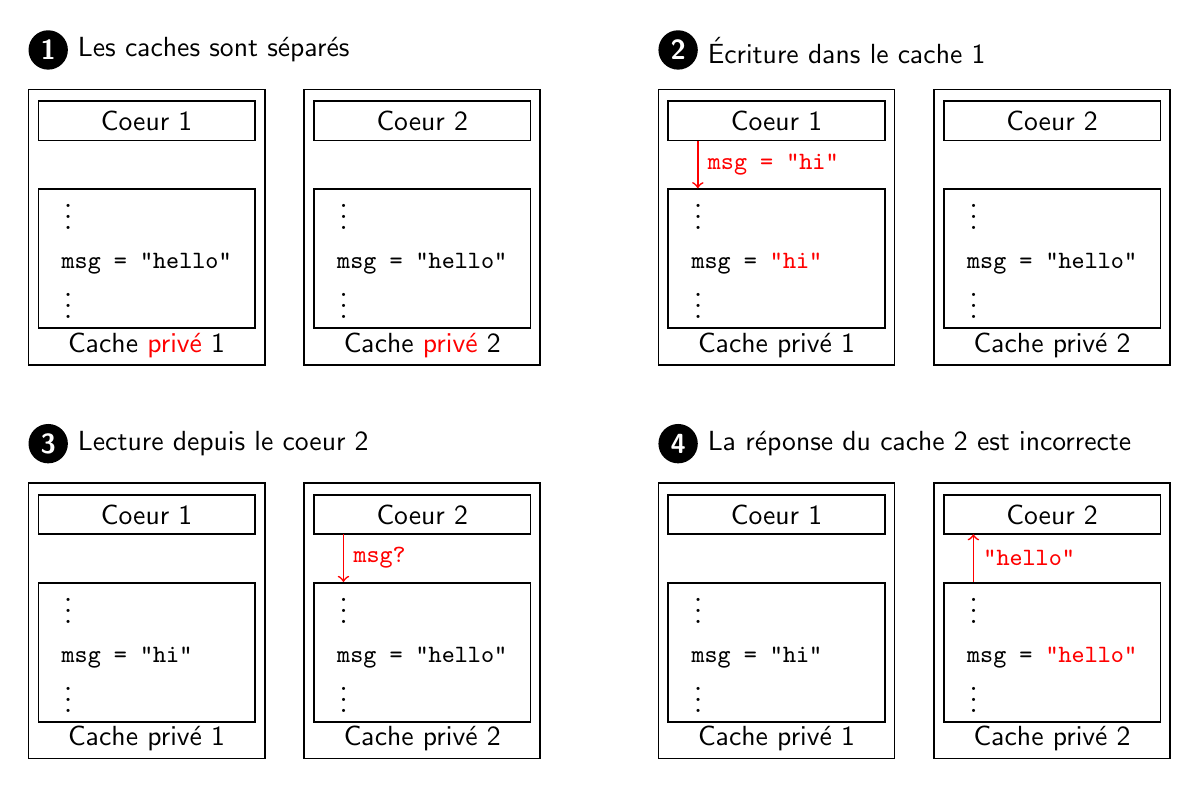
\begin{tikzpicture}
    \begin{scope}[shift={(0,0)}]
      \fill[black] (0.25,4) circle (0.25) node[white,font=\bf] {1};
      \draw (0.5, 4) node[right] {Les caches sont séparés};
      \begin{scope}[shift={(0,0)}]
        \draw (0,0) rectangle ++(3,3.5);
        \draw (1.5,3.1) node[draw,minimum width=2.75cm,minimum height=0.5cm] {Coeur 1};
        \node[draw,align=left,font=\small\tt,minimum width=2.75cm] (CACHE1) at (1.5,1.35) {~\\[-0.5em] $\vdots$ \\[3pt] msg = "hello" \\ $\vdots$};
        \draw (1.5,0.25) node {Cache \textcolor{red}{privé} 1};
      \end{scope}
      \begin{scope}[shift={(3.5,0)}]
        \draw (0,0) rectangle ++(3,3.5);
        \draw (1.5,3.1) node[draw,minimum width=2.75cm,minimum height=0.5cm] {Coeur 2};
        \node[draw,align=left,font=\small\tt,minimum width=2.75cm] (CACHE2) at (1.5,1.35) {~\\[-0.5em] $\vdots$ \\[3pt] msg = "hello" \\ $\vdots$};
        \draw (1.5,0.25) node {Cache \textcolor{red}{privé} 2};
      \end{scope}
    \end{scope}

    \begin{scope}[shift={(8,0)}]
      \fill[black] (0.25,4) circle (0.25) node[white,font=\bf] {2};
      \draw (0.5, 4) node[right] {Écriture dans le cache 1};
      \begin{scope}[shift={(0,0)}]
        \draw (0,0) rectangle ++(3,3.5);
        \draw (1.5,3.1) node[draw,minimum width=2.75cm,minimum height=0.5cm] {Coeur 1};
        \node[draw,align=left,font=\small\tt,minimum width=2.75cm] (CACHE1) at (1.5,1.35) {~\\[-0.5em] $\vdots$ \\[3pt] msg = \textcolor{red}{"hi"}~~~~ \\ $\vdots$};
        \draw (1.5,0.25) node {Cache privé 1};
        \draw[red,->] (0.5,2.85) -- node[right] {\small\tt msg = "hi"} ([xshift=-1cm] CACHE1.north);
      \end{scope}
      \begin{scope}[shift={(3.5,0)}]
        \draw (0,0) rectangle ++(3,3.5);
        \draw (1.5,3.1) node[draw,minimum width=2.75cm,minimum height=0.5cm] {Coeur 2};
        \node[draw,align=left,font=\small\tt,minimum width=2.75cm] (CACHE2) at (1.5,1.35) {~\\[-0.5em] $\vdots$ \\[3pt] msg = "hello" \\ $\vdots$};
        \draw (1.5,0.25) node {Cache privé 2};
      \end{scope}
    \end{scope}

    \begin{scope}[shift={(0,-5)}]
      \fill[black] (0.25,4) circle (0.25) node[white,font=\bf] {3};
      \draw (0.5, 4) node[right] {Lecture depuis le coeur 2};
      \begin{scope}[shift={(0,0)}]
        \draw (0,0) rectangle ++(3,3.5);
        \draw (1.5,3.1) node[draw,minimum width=2.75cm,minimum height=0.5cm] {Coeur 1};
        \node[draw,align=left,font=\small\tt,minimum width=2.75cm] (CACHE1) at (1.5,1.35) {~\\[-0.5em] $\vdots$ \\[3pt] msg = "hi"~~~~ \\ $\vdots$};
        \draw (1.5,0.25) node {Cache privé 1};
      \end{scope}
      \begin{scope}[shift={(3.5,0)}]
        \draw (0,0) rectangle ++(3,3.5);
        \draw (1.5,3.1) node[draw,minimum width=2.75cm,minimum height=0.5cm] {Coeur 2};
        \node[draw,align=left,font=\small\tt,minimum width=2.75cm] (CACHE2) at (1.5,1.35) {~\\[-0.5em] $\vdots$ \\[3pt] msg = "hello" \\ $\vdots$};
        \draw (1.5,0.25) node {Cache privé 2};
        \draw[red,->] (0.5,2.85) -- node[right] {\small\tt msg?} ([xshift=-1cm] CACHE2.north);
      \end{scope}
    \end{scope}

    \begin{scope}[shift={(8,-5)}]
      \fill[black] (0.25,4) circle (0.25) node[white,font=\bf] {4};
      \draw (0.5, 4) node[right] {La réponse du cache 2 est incorrecte};
      \begin{scope}[shift={(0,0)}]
        \draw (0,0) rectangle ++(3,3.5);
        \draw (1.5,3.1) node[draw,minimum width=2.75cm,minimum height=0.5cm] {Coeur 1};
        \node[draw,align=left,font=\small\tt,minimum width=2.75cm] (CACHE1) at (1.5,1.35) {~\\[-0.5em] $\vdots$ \\[3pt] msg = "hi"~~~~ \\ $\vdots$};
        \draw (1.5,0.25) node {Cache privé 1};
      \end{scope}
      \begin{scope}[shift={(3.5,0)}]
        \draw (0,0) rectangle ++(3,3.5);
        \draw (1.5,3.1) node[draw,minimum width=2.75cm,minimum height=0.5cm] {Coeur 2};
        \node[draw,align=left,font=\small\tt,minimum width=2.75cm] (CACHE2) at (1.5,1.35) {~\\[-0.5em] $\vdots$ \\[3pt] msg = \textcolor{red}{"hello"} \\ $\vdots$};
        \draw (1.5,0.25) node {Cache privé 2};
        \draw[red,<-] (0.5,2.85) -- node[right] {\small\tt "hello"} ([xshift=-1cm] CACHE2.north);
      \end{scope}
    \end{scope}
  \end{tikzpicture}
\end{document}
